%%***( Diseño sistema base )********************************************************

%%==================================================================================

\section{Diagrama de contexto}

El proyecto cuenta con el siguiente diagrama de contexto:

\begin{figure}[h]
    \centering
    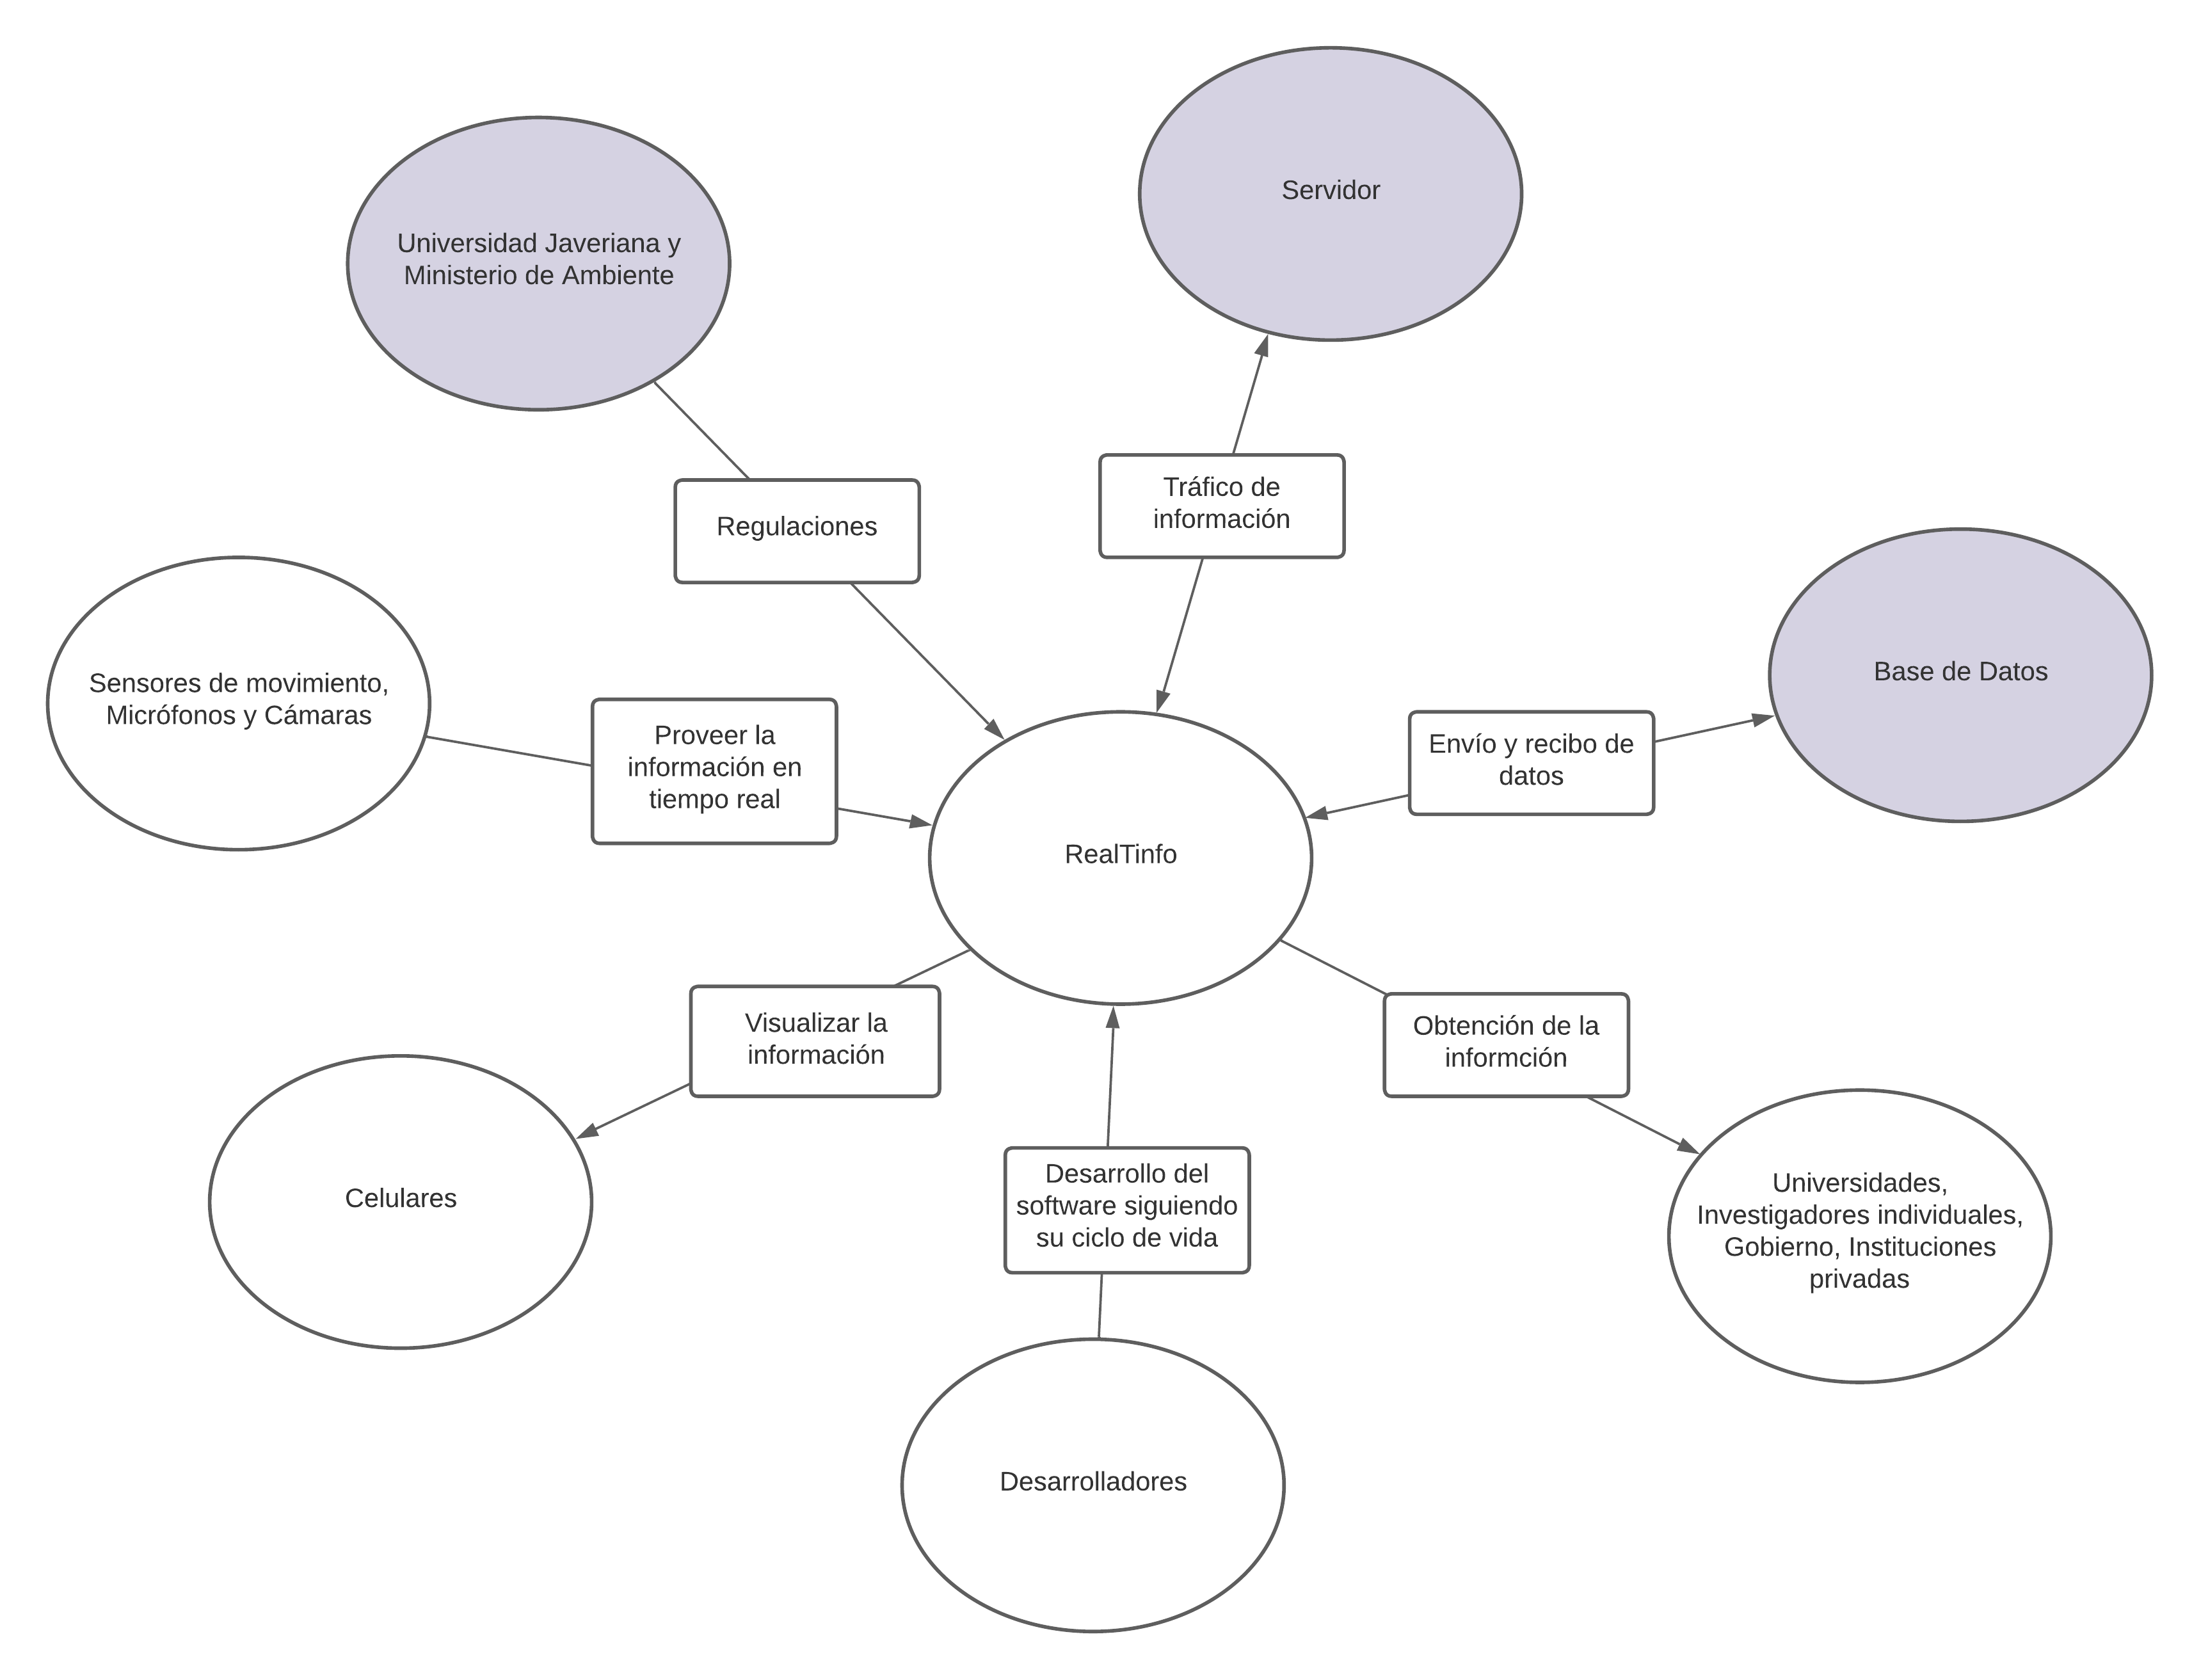
\includegraphics[width=0.90\textwidth]{images/Diagrama de Contexto.png}
    \caption{Diagrama de Contexto.}
    \label{diag_cont}
\end{figure}

El sistema tiene varios actores dentro del diagrama, las razones por las cuales están estos actores son:

\begin{itemize}
    \item Las regulaciones están dadas por el Ministerio de Ambiente y la Pontificia Universidad Javeriana Cali, ya que son las principales entidades que limitarán el proyecto con respecto a las restricciones para un correcto desarrollo y ejecución.
    \item El servidor funciona como un dispositivo que se encuentra en la nube y funciona por medio de internet para pasar la información entre la base de datos, los dispositivos de cómputo y los dispositivos para la toma de la información.
    \item La base de datos se va a usar para guardar la información que es transmitida.
    \item Las universidades, investigadores individuales, gobierno, etc. Son los usuarios finales a los cuales potencialmente se les puede transmitir la información.
    \item Los desarrolladores se encargan de diseñar el sistema y revisar su funcionamiento.
    \item Los celulares son los dispositivos de cómputo que van a recibir la información de la base de datos que soliciten.
    \item Por último, están los dispositivos que toma la información y la transmiten.
\end{itemize}

%%==================================================================================
\section{Diagramas MSC en el nivel de sistema}

El diagrama MSC se compone de varias partes, la primera parte es la siguiente:

\begin{figure}[h]
    \centering
    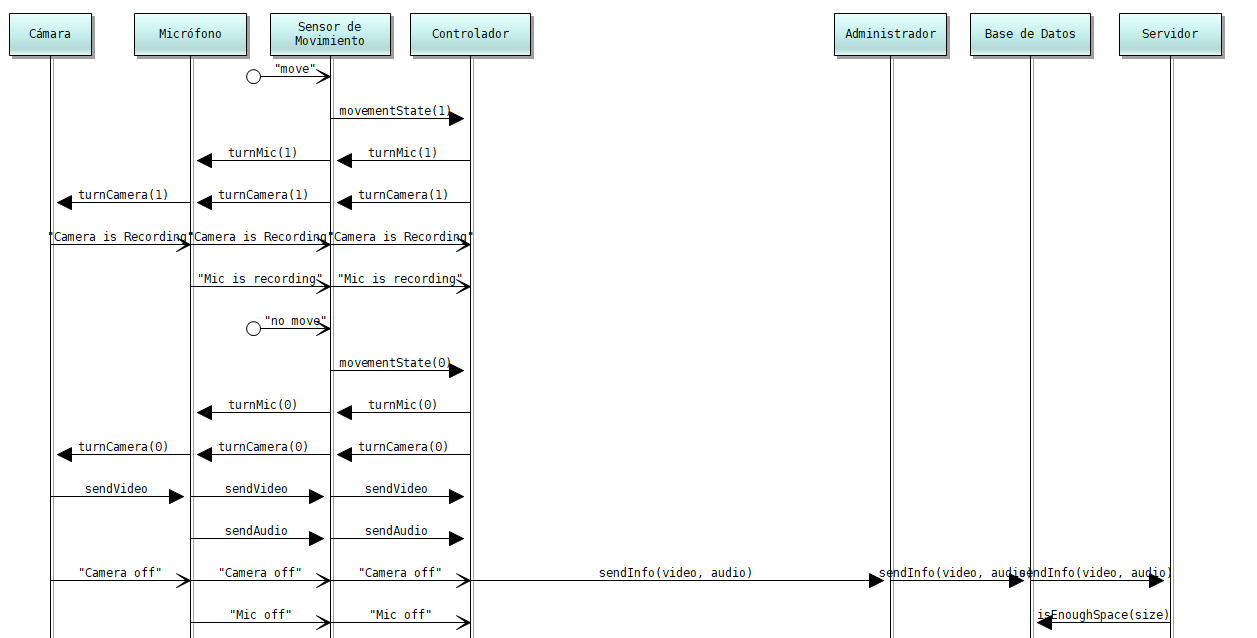
\includegraphics[width=0.90\textwidth]{images/MSC1.png}
    \caption{Diagrama Message Sequence Chart (MSC).}
    \label{MSC1}
\end{figure}

\begin{figure}[h]
    \centering
    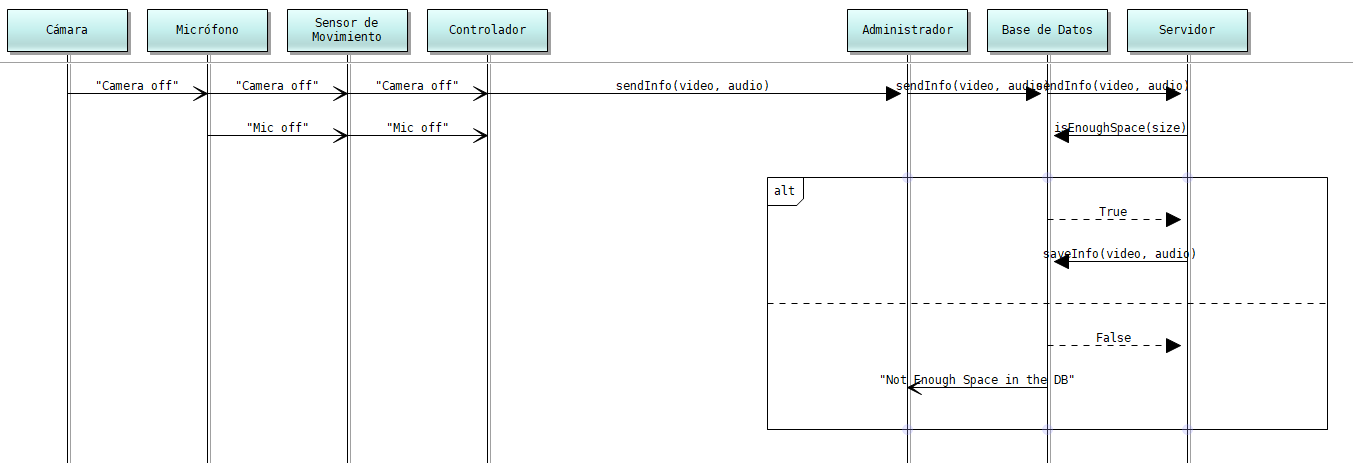
\includegraphics[width=0.90\textwidth]{images/MSC2.png}
    \caption{Diagrama Message Sequence Chart (MSC).}
    \label{MSC2}
\end{figure}

\pagebreak

En esta primera parte en las figuras (\ref{MSC1}) y (\ref{MSC2}), funciona cuando se activa el trigger de movimiento en el sensor de movimiento, cuando esto es activado se envía una señal al controlador y el controlador ordena prender los dispositivos para que empiecen a grabar, una vez que el movimiento se detiene, después de un timer que tiene el sensor de movimiento, se manda una señal para indicar que no hay movimiento al controlador y por ende ordenar apagar la cámara y el micrófono, pero antes estos envían lo grabado para ser almacenado en la base de datos.

En la base de datos se verifica si hay espacio, si hay espacio las grabaciones se guardan y cuando no se pierden. Al mismo tiempo que ocurre lo anterior se apagan los dispositivos para ahorrar su energía.

\begin{figure}[h]
    \centering
    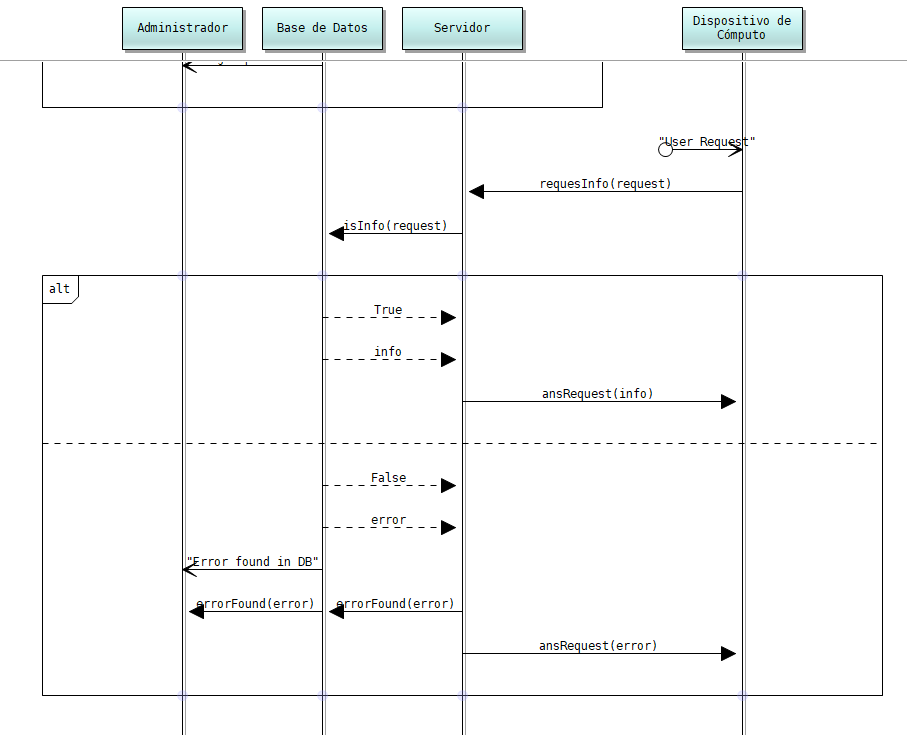
\includegraphics[width=0.70\textwidth]{images/MSC3.png}
    \caption{Diagrama Message Sequence Chart (MSC).}
    \label{MSC3}
\end{figure}

En esta parte del diagrama se muestra cuando un usuario hace una solicitud para obtener la información del sistema, cuando se pide la solicitud se revisa en la base de datos dos casos: 1) si la información solicitada está, entonces le avisa al servidor que es correcto, entonces se envía la información al usuario para que le sea desplegada, 2) el segundo caso es cuando la información solicitada tiene algún error (no se encuentra, está corrupta, etc.), este error se el envía a un administrador del sistema y se le muestra al usuario que ocurrió un error y la razón.

\begin{figure}[h]
    \centering
    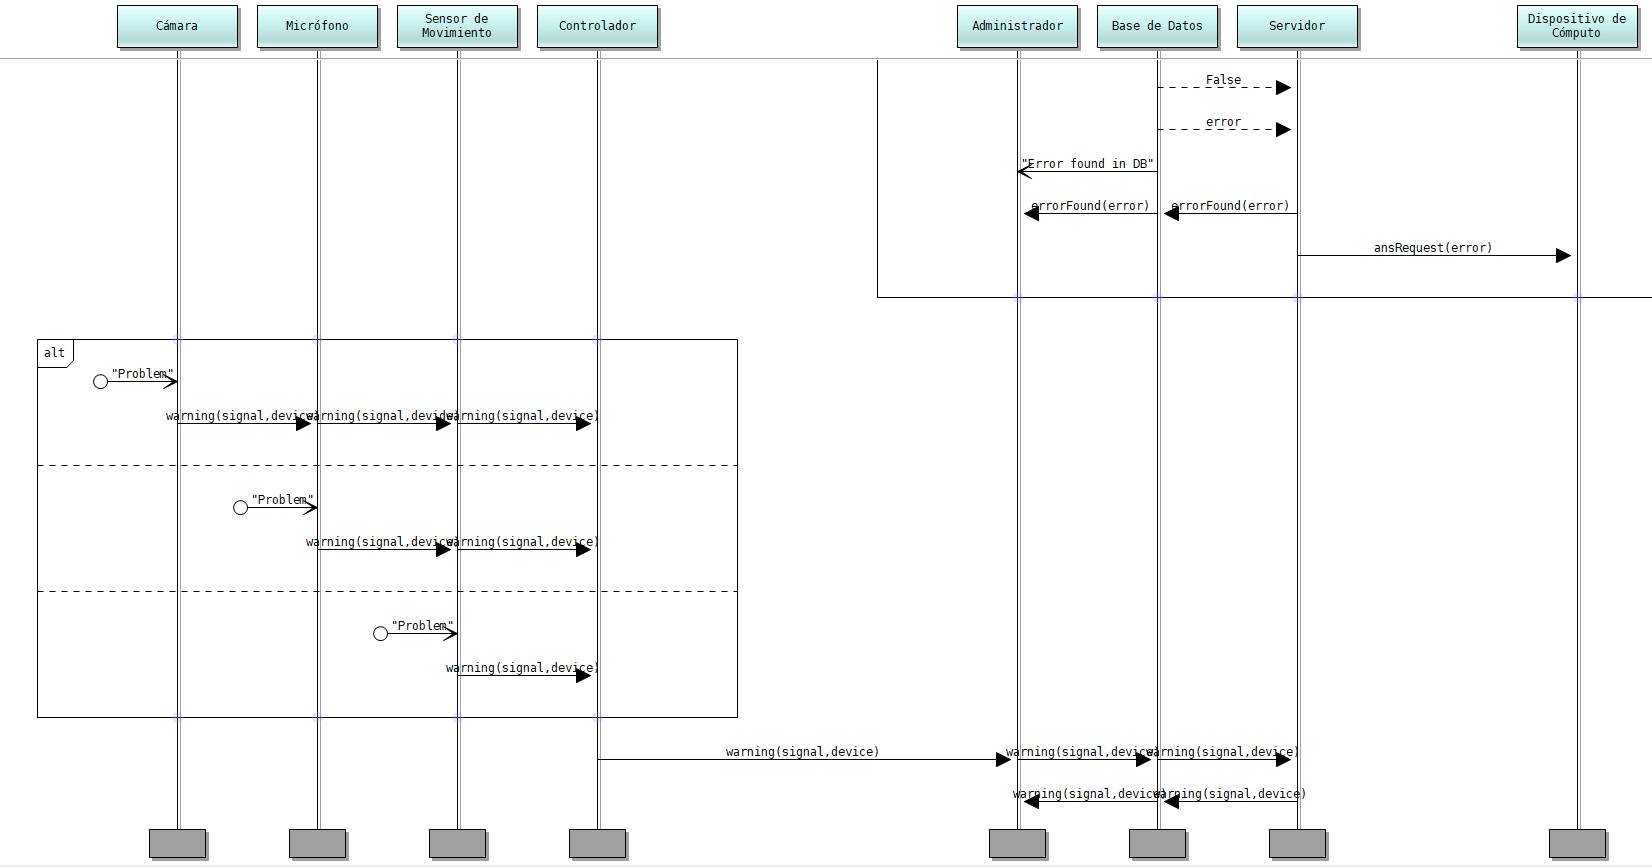
\includegraphics[width=0.90\textwidth]{images/MSC4.png}
    \caption{Diagrama Message Sequence Chart (MSC).}
    \label{MSC4}
\end{figure}

En esta parte del diagrama se muestra cuando ocurre un problema con los dispositivos de la toma de información, ocurren varios casos:

\begin{itemize}
    \item La primera es cuando la cámara tiene un problema por la temperatura, por la batería o el almacenamiento interno de la misma, en cualquiera de los casos se envía una señal y el dispositivo hacia el controlador.
    \item La segunda es cuando el micrófono no tiene batería suficiente o tiene más almacenamiento, en estos caso se le envía una señal y el dispositivo al controlador.
    \item Por último, si el sensor de movimiento presenta algún tipo de problema este va a enviar una señal y el dispositivo al controlador
\end{itemize}

Cuando cualquier señal es enviada al controlador este envía el dispositivo que la envío y el problema (la señal) al administrador para que haga el debido proceso para hacerse cargo de este problema.

%%==================================================================================
\section{Arquitectura SDL y procesos}
Después de haber realizado los diagramas MSC, se pasó a realizar el diagrama SDL sobre la arquitectura y comunicación del sistema, en donde se muestran las interacciones entre las señales con los bloques y procesos generados del sistema.

Primeramente, el sistema cuenta con una arquitectura general y una sección de declaraciones con respecto a las señales, tipos y variables globales, es decir, que se pueden acceder en cualquier sección de la arquitectura, (ver figura \ref{SDL_General})

\begin{figure}[h]
    \centering
    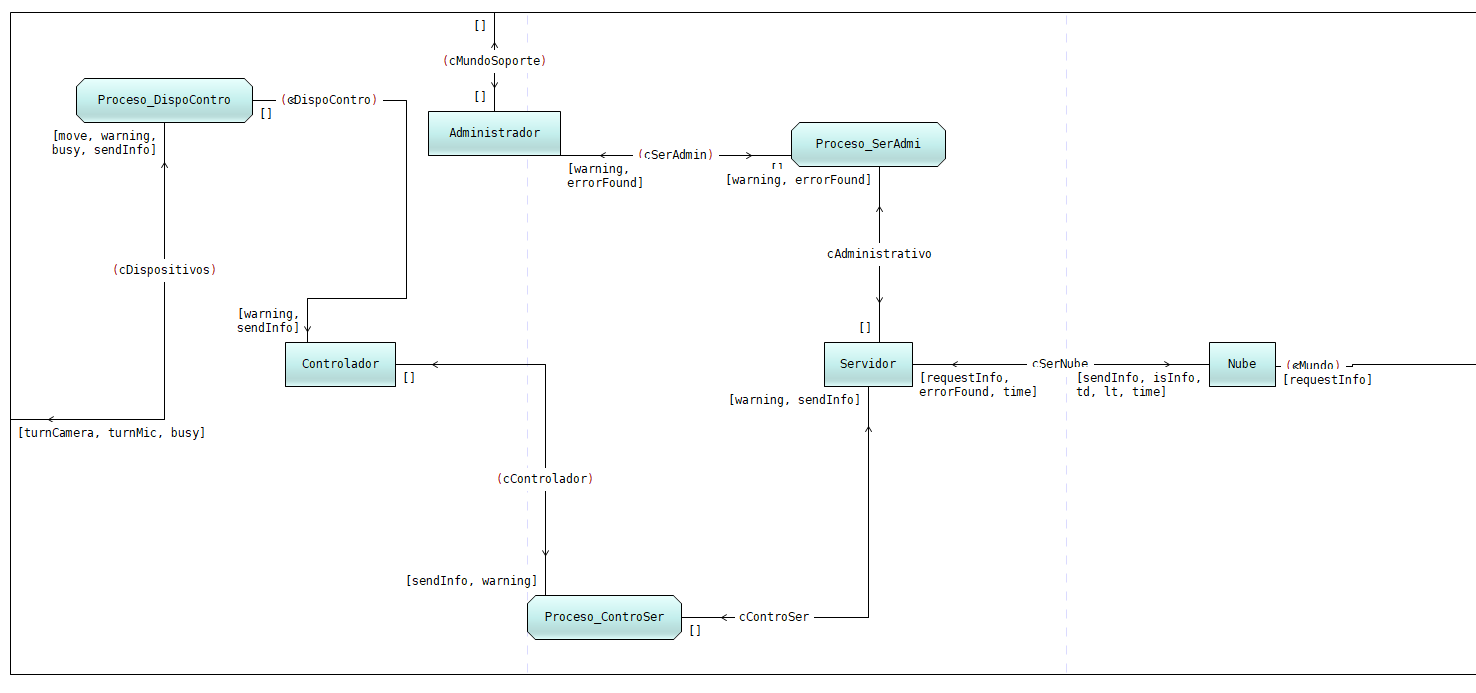
\includegraphics[width=0.95\textwidth]{images/SDL_General1.png}
    \caption{Diagrama SDL}
    \label{SDL_General}
\end{figure}

Como se puede observar, tiene varios canales para el paso de mensajes y se comunica entre procesos y bloques para el manejo de la información que se solicita.

\begin{figure}[h]
    \centering
    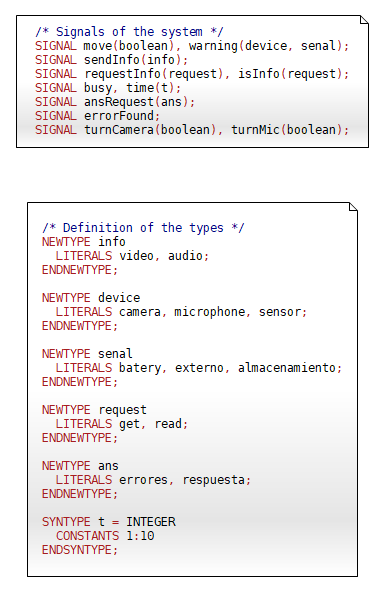
\includegraphics[width=0.5\textwidth]{images/SDL_GeneralDeclaraciones.png}
    \caption{Diagrama SDL (declaraciones)}
    \label{SDL_GeneralDeclaraciones}
\end{figure}

\pagebreak

Además, en la figura \ref{SDL_GeneralDeclaraciones}, por la parte de las declaraciones, se tienen las señales que manejan la información de manera global en cualquier parte de la arquitectura. También, cuenta con los tipos de datos que manejan las señales. En las declaraciones se muestran las señales con el tipo de parámetro que lleva, si es que llevan. \\

Por otro lado, el proceso entre los dispositivos y el controlador, se puede observar que se encarga de manejar la información que se transmite entre los dispositivos y el controlado general, ya que pueden haber errores o la información tomada.

\begin{figure}[h]
    \centering
    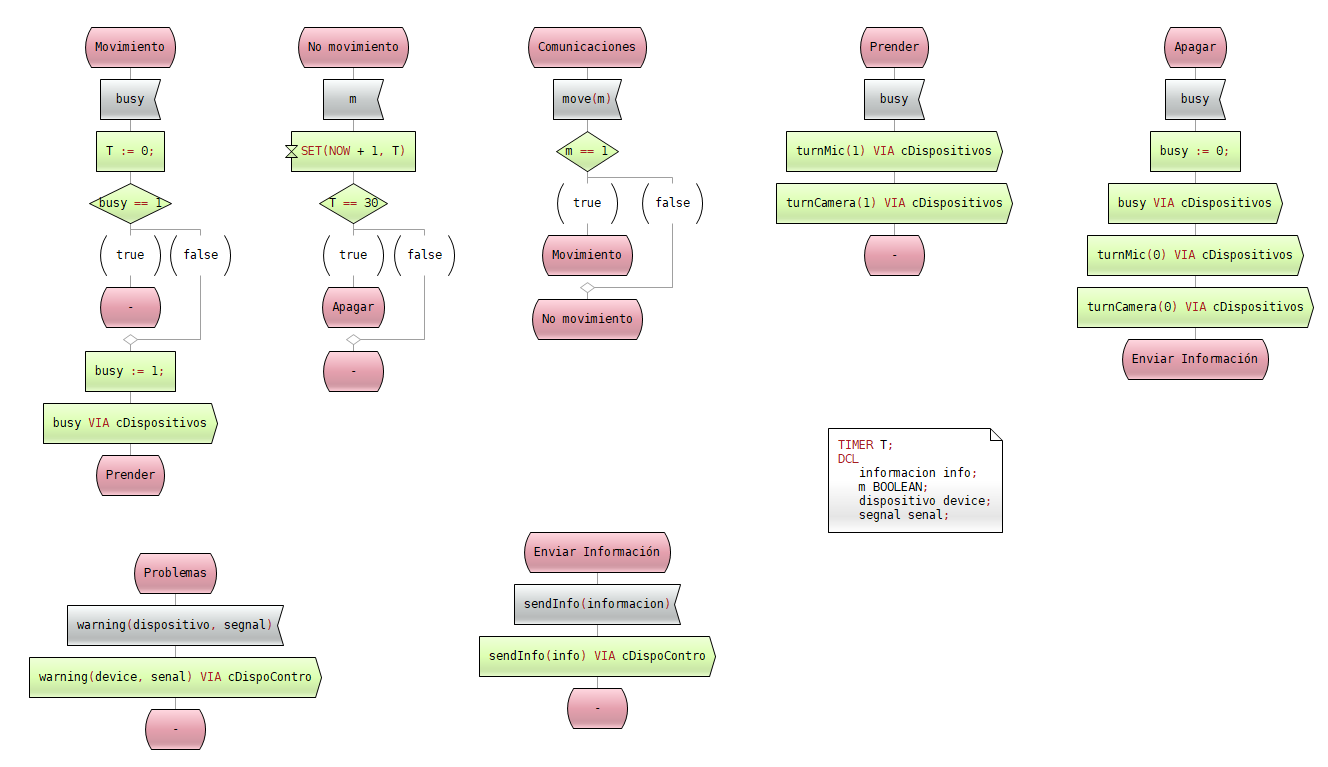
\includegraphics[width=0.9\textwidth]{images/SDL_ProcesoDipoContro.png}
    \caption{Diagrama SDL Proceso Dispositivos-Controlador}
    \label{SDL_PdispoContro}
\end{figure}

\pagebreak

En la figura \ref{SDL_PdispoContro} se puede ver que hay distintos estados en donde se maneja el paso de la información (problemas o datos grabados), además se tiene un estado para determinar si un animal se encuentra en movimiento o no, con esto se pueden grabar con mayor facilidad los datos y no va a haber problemas con otras señales ya que el canal va a estar ocupado. Entonces, si el canal se encuentra ocupado es porque los dispositivos están grabando, está desocupado en caso contrario.

Para determinar el tiempo que se graba, se tiene un temporizador que va a medir el tiempo de grabación para tomar los datos, cuando se cumpla ese tiempo, los dispositivos se apagan para ahorrar energía, ya que no pueden estar prendidos todo el tiempo.

\begin{figure}[h]
    \centering
    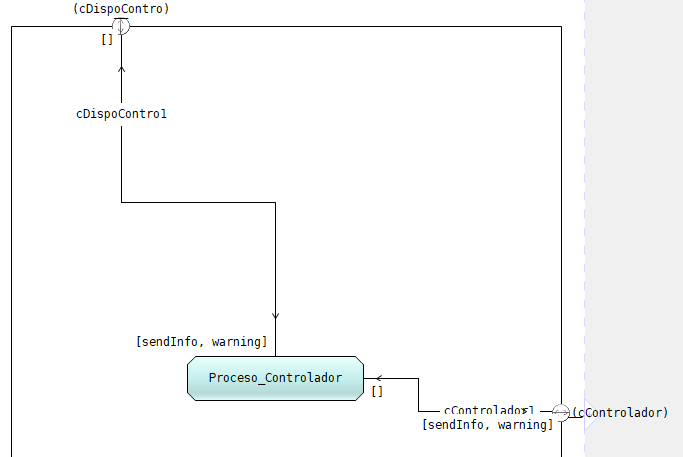
\includegraphics[width=0.7\textwidth]{images/SDL_Controlador.png}
    \caption{Diagrama SDL del Controlador}
    \label{SDL_Controlador}
\end{figure}

\pagebreak

Dentro del controlador solo se encuentra un proceso que maneja la información que se pasa, ya que la distribuye hasta el servidor. Dentro del proceso se encuentra un diagrama que muestra como recibe la información y como la envía en la figura \ref{SDL_PcontroSer}.

\begin{figure}[h]
    \centering
    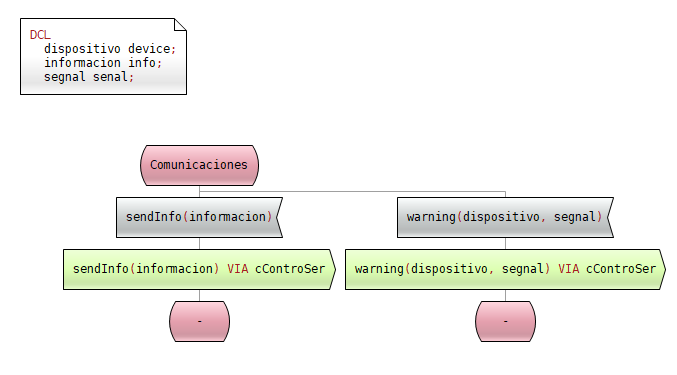
\includegraphics[width=0.8\textwidth]{images/SDL_ProcesoControSer.png}
    \caption{Diagrama SDL del Proceso dentro del controlador}
    \label{SDL_Pcontro}
\end{figure}

Luego, viene el proceso que conecta el controlador con el servidor, de hecho, hace el mismo proceso que el proceso dentro del controlador (ver la figura \ref{SDL_PcontroSer}).

\begin{figure}[h]
    \centering
    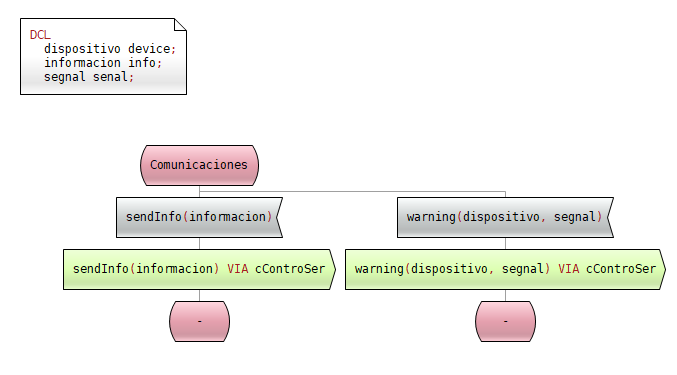
\includegraphics[width=0.9\textwidth]{images/SDL_ProcesoControSer.png}
    \caption{Diagrama SDL del Proceso que conecta el controlador con el Servidor.}
    \label{SDL_PcontroSer}
\end{figure}

\pagebreak

Ahora bien, en la parte del servidor encuentra un único proceso que conecta con tres secciones: administrador, controlador y la nube (ver la figura \ref{SDL_Servidor}).

\begin{figure}[h]
    \centering
    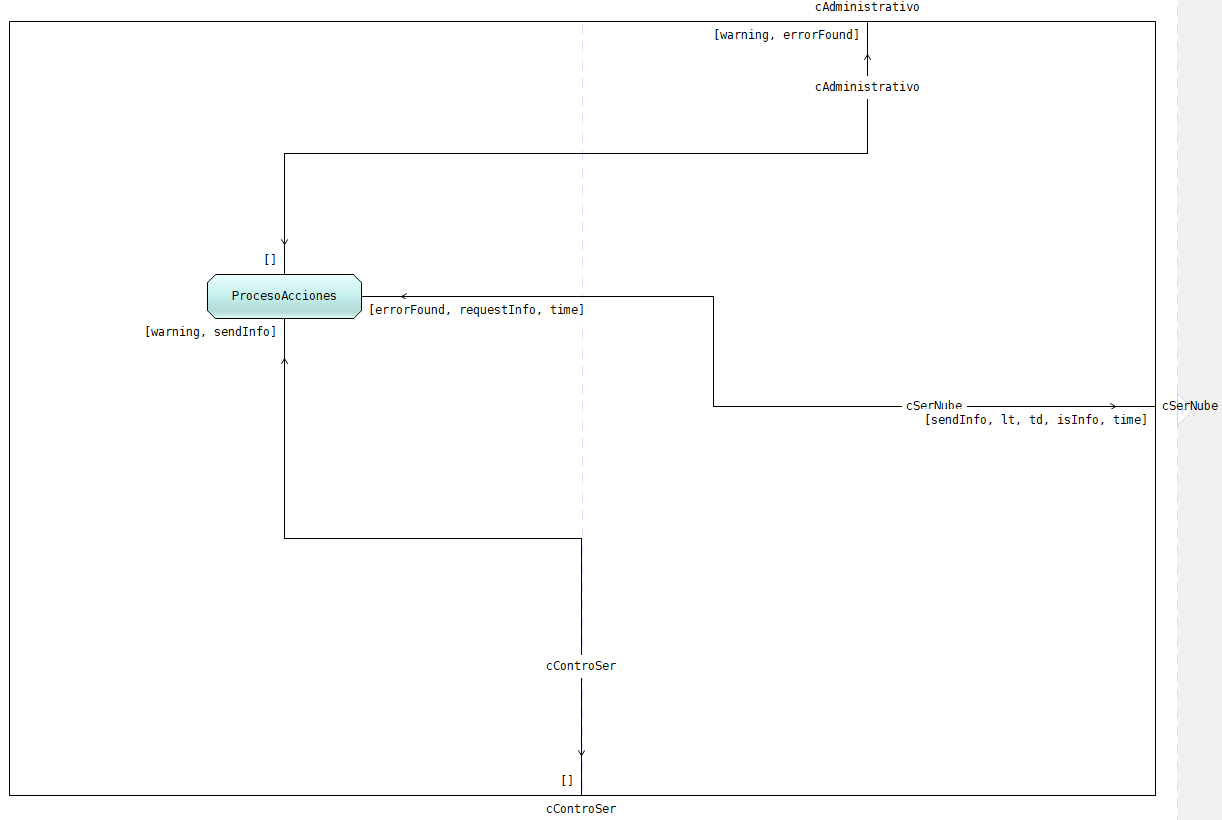
\includegraphics[width=0.65\textwidth]{images/SDL_Servidor.png}
    \caption{Diagrama SDL del Servidor}
    \label{SDL_Servidor}
\end{figure}

\pagebreak

\begin{figure}[h]
    \centering
    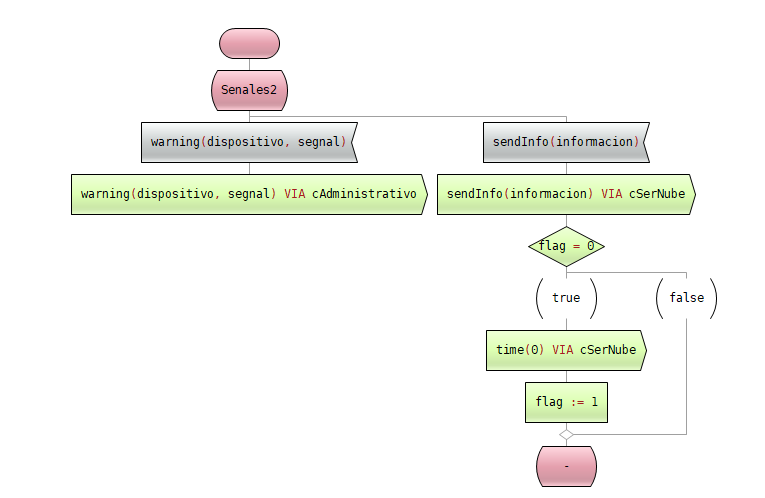
\includegraphics[width=0.8\textwidth]{images/SDL_ProcesoAcciones1.png}
    \caption{Diagrama SDL del Proceso dentro del Servidor (parte 1)}
    \label{SDL_Pservidor1}
\end{figure}

\begin{figure}[h]
    \centering
    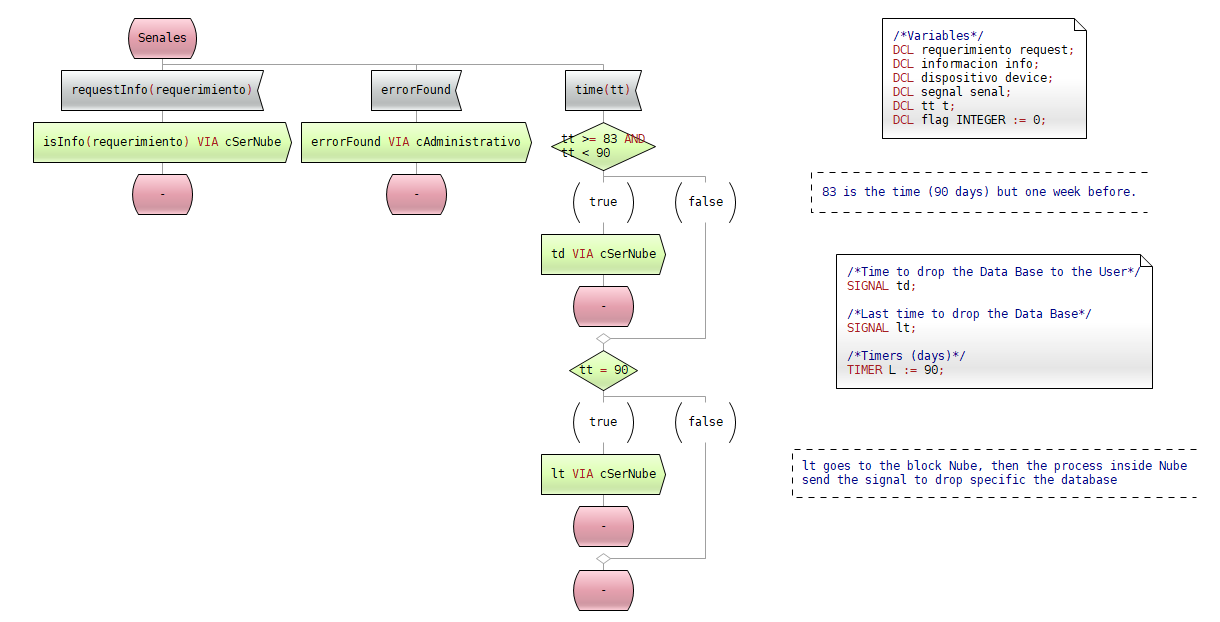
\includegraphics[width=0.8\textwidth]{images/SDL_ProcesoAcciones2.png}
    \caption{Diagrama SDL del Proceso dentro del Servidor (parte 2)}
    \label{SDL_Pservidor2}
\end{figure}

En las figuras \ref{SDL_Pservidor1} y \ref{SDL_Pservidor2} se muestran los estados para pasar las señales (errores o datos) hasta administrador o hasta la nube. Además, el servidor se encarga de contar el tiempo (periodo) con el que cuentan los usuarios para hacer uso del sistema, ya que después de cumplir el tiempo la base de datos eliminará la información que tiene almacenada.

Es por eso, que el servidor se encarga de avisar al usuario cuando le quede una semana, con esto el usuario cuenta con una semana para descargar la información o guardarla en otra parte, si en el tiempo en el que tuvo para eso no descargó la información ya no tendrá acceso ni oportunidad para obtenerlas. Esto se hace con el propósito de que la base de datos no se llene en algún momento y se pueda prevenir esos errores, para seguir almacenando la información sin problemas.

Cuando se cumpla el tiempo de una semana antes de que se venza el periodo que tienen se va a enviar una señal al usuario para avisar que se va a eliminar, cuando se venza todo el plazo después de una semana de antelación, se envía una señal a la base de datos para borrar la información. \\

En la figura \ref{SDL_PserAdmin}, se ve el proceso que conecta el servidor con el administrador, el cual se encarga solamente de pasar la información hasta el administrador.

\begin{figure}[h]
    \centering
    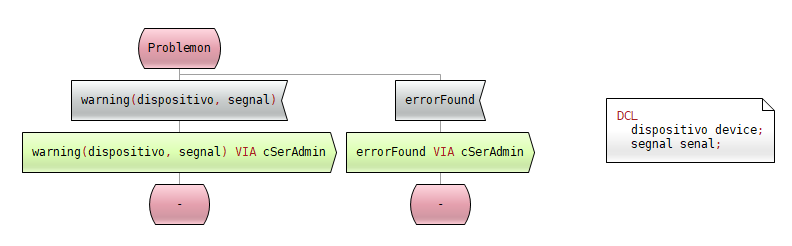
\includegraphics[width=0.8\textwidth]{images/SDL_ProcesoSerAdmi.png}
    \caption{Diagrama SDL del Proceso entre el Servidor y el Administrador}
    \label{SDL_PserAdmin}
\end{figure}

En las figuras \ref{SDL_Admin} y \ref{SDL_Padmin}, se ve el proceso que está dentro del administrador y lo que se encarga de hacer, que es el paso de la información hacia el mundo (internet) y lo que manejan como administradores, que reciben los errores y logs de la nube.

\begin{figure}[h]
    \centering
    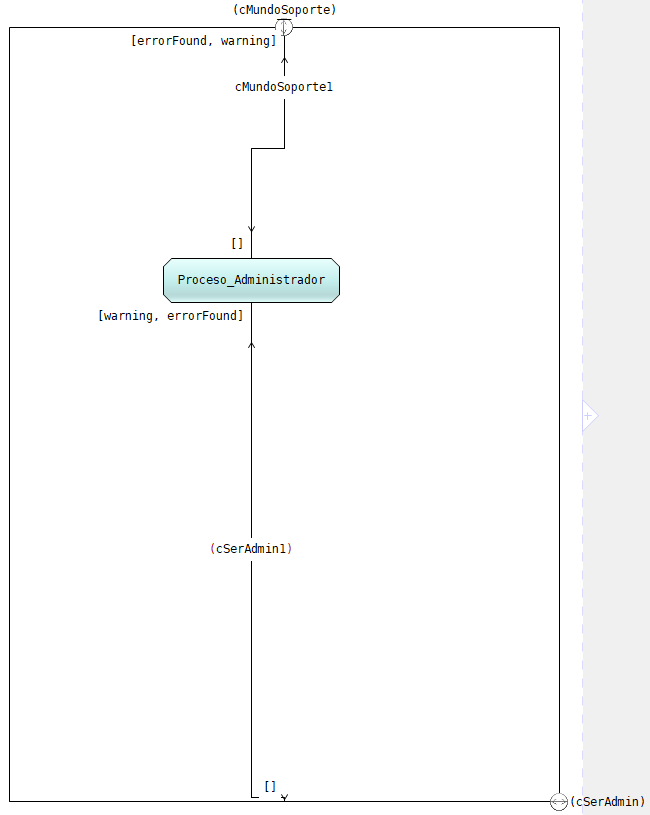
\includegraphics[width=0.45\textwidth]{images/SDL_Administrador.png}
    \caption{Diagrama SDL del Administrador}
    \label{SDL_Admin}
\end{figure}

\begin{figure}[h]
    \centering
    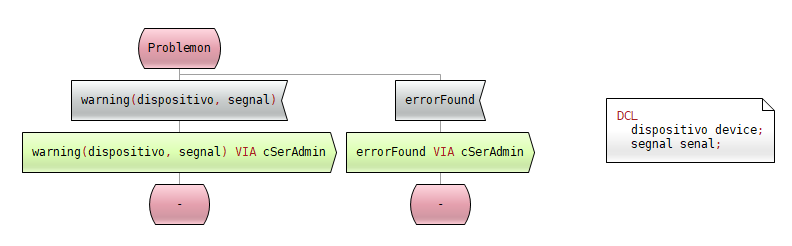
\includegraphics[width=0.9\textwidth]{images/SDL_ProcesoSerAdmi.png}
    \caption{Diagrama SDL del Proceso dentro del Administrador}
    \label{SDL_Padmin}
\end{figure}

Por último, se encuentra el bloque de la nube (ver la figura \ref{SDL_Nube}), este bloque contiene un proceso para manejar la información entre el servidor y el usuario con la base de datos. Además, la nube con tiene más cosas que se pueden hacer con los datos en un nivel más específico como el uso de Inteligencia Artificial, sin embargo, no es necesario hacerlo para el contexto de este proyecto.

\begin{figure}[h]
    \centering
    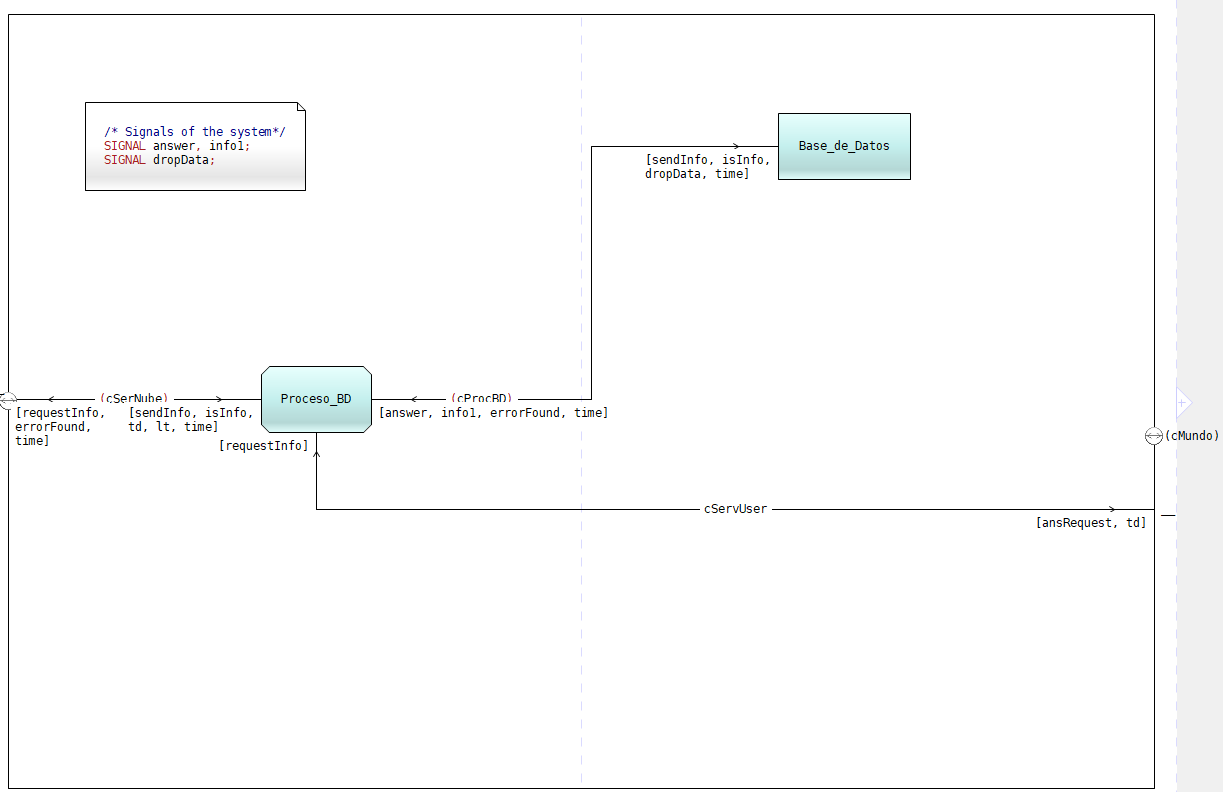
\includegraphics[width=0.8\textwidth]{images/SDL_Nube.png}
    \caption{Diagrama SDL de la Nube}
    \label{SDL_Nube}
\end{figure}

Dentro del proceso (figura \ref{SDL_Pnube}) se reciben señales y envían a los diferentes canales dependiendo de la señal ya sea para guardar la información, para avisar al usuario de borrar la base de datos, para borrar la base de datos o para verificar una petición que llegue por parte del usuario, pero, cuando se trata de la petición esta puede tener dos valores, que sea falsa o verdadera, en caso de ser verdadera retorna al usuario lo que solicitó y en caso de ser falsa retorna el error al usuario y al administrador.

\begin{figure}[h]
    \centering
    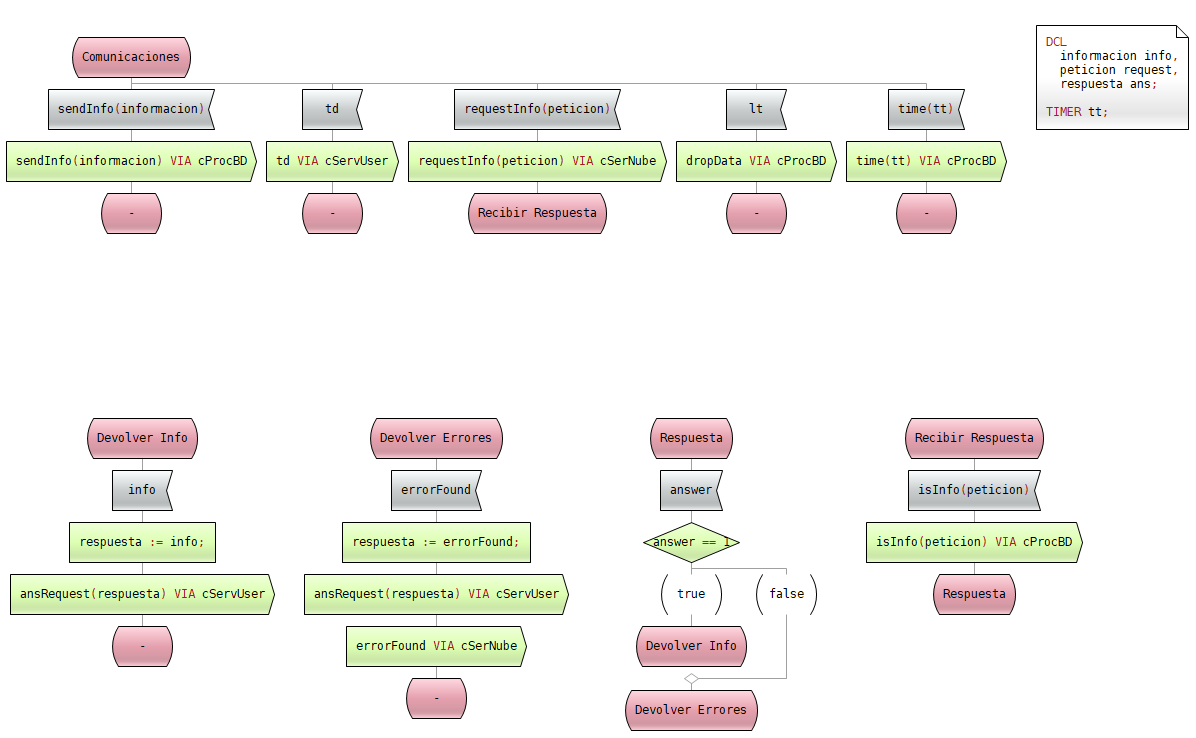
\includegraphics[width=0.9\textwidth]{images/SDL_ProcesoBD.png}
    \caption{Diagrama SDL del Proceso dentro de la Nube}
    \label{SDL_Pnube}
\end{figure}

En la última parte, se encuentra la base de datos que contiene un proceso para responder a la información que se pide (figura \ref{SDL_BaseDeDatos}). En dicho proceso, se guarda la información que se recibe y se da una respuesta dependiendo si el requerimiento es correcto o no y además, el tiempo que se cuenta para evaluar el periodo (ver figura \ref{SDL_Pbd}).

\begin{figure}[h]
    \centering
    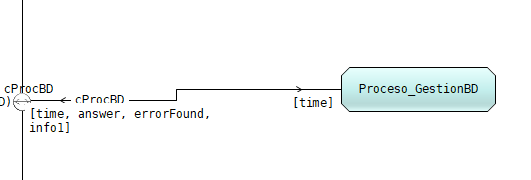
\includegraphics[width=0.8\textwidth]{images/SDL_BaseDeDatos.png}
    \caption{Diagrama SDL de la Base de Datos}
    \label{SDL_BaseDeDatos}
\end{figure}

\begin{figure}[h]
    \centering
    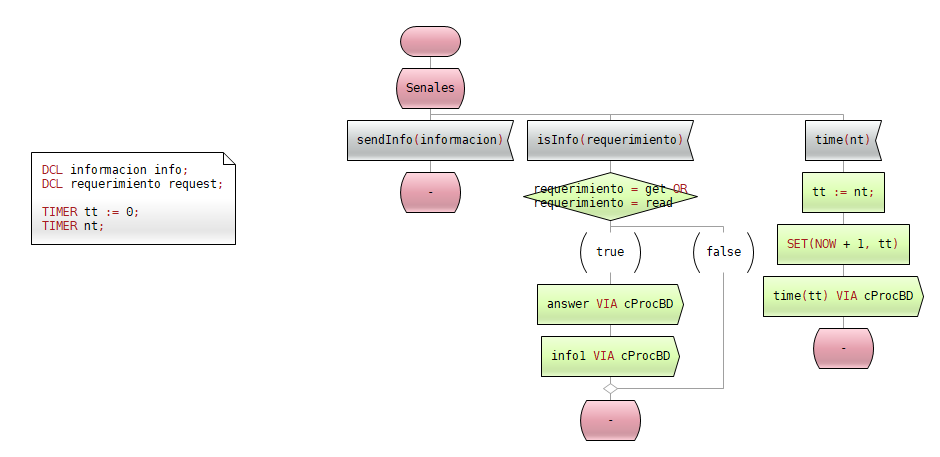
\includegraphics[width=0.8\textwidth]{images/SDL_ProcesoGestionBD.png}
    \caption{Diagrama SDL del Proceso dentro de la Base de Datos}
    \label{SDL_Pbd}
\end{figure}

\pagebreak

Aunque se muestra el diagrama SDL, aún tiene fallas y faltan cosas por terminar para hacer el plan de pruebas, ya que al no poder solucionar los errores no se hizo la ejecución del plan de pruebas.

%%==================================================================================
\begin{comment}
\section{Evaluación de alternativas de diseño}

    Describa las alternativas propuestas para el diseño de cada subsistema (entre las que se incluyan propuestas propias).\\
    
    Presente el proceso de selección de la mejor alternativa para el diseño de cada subsistema, a partir de la evaluación del cumplimiento de todas las especificaciones funcionales en el marco de las restricciones del proyecto.\\
    
    Describa claramente los criterios de diseño y selección utilizados.
\end{comment}
%%==================================================================================
\section{Verificación del sistema base}

    Presente el plan de pruebas (escenarios y casos de prueba) y los resultados de las diferentes pruebas realizadas al diseño (trazas de ejecución MSC) con los que se muestra la validez del diseño frente a los requerimientos definidos previamente.

\begin{figure}[!h]
    \centering
    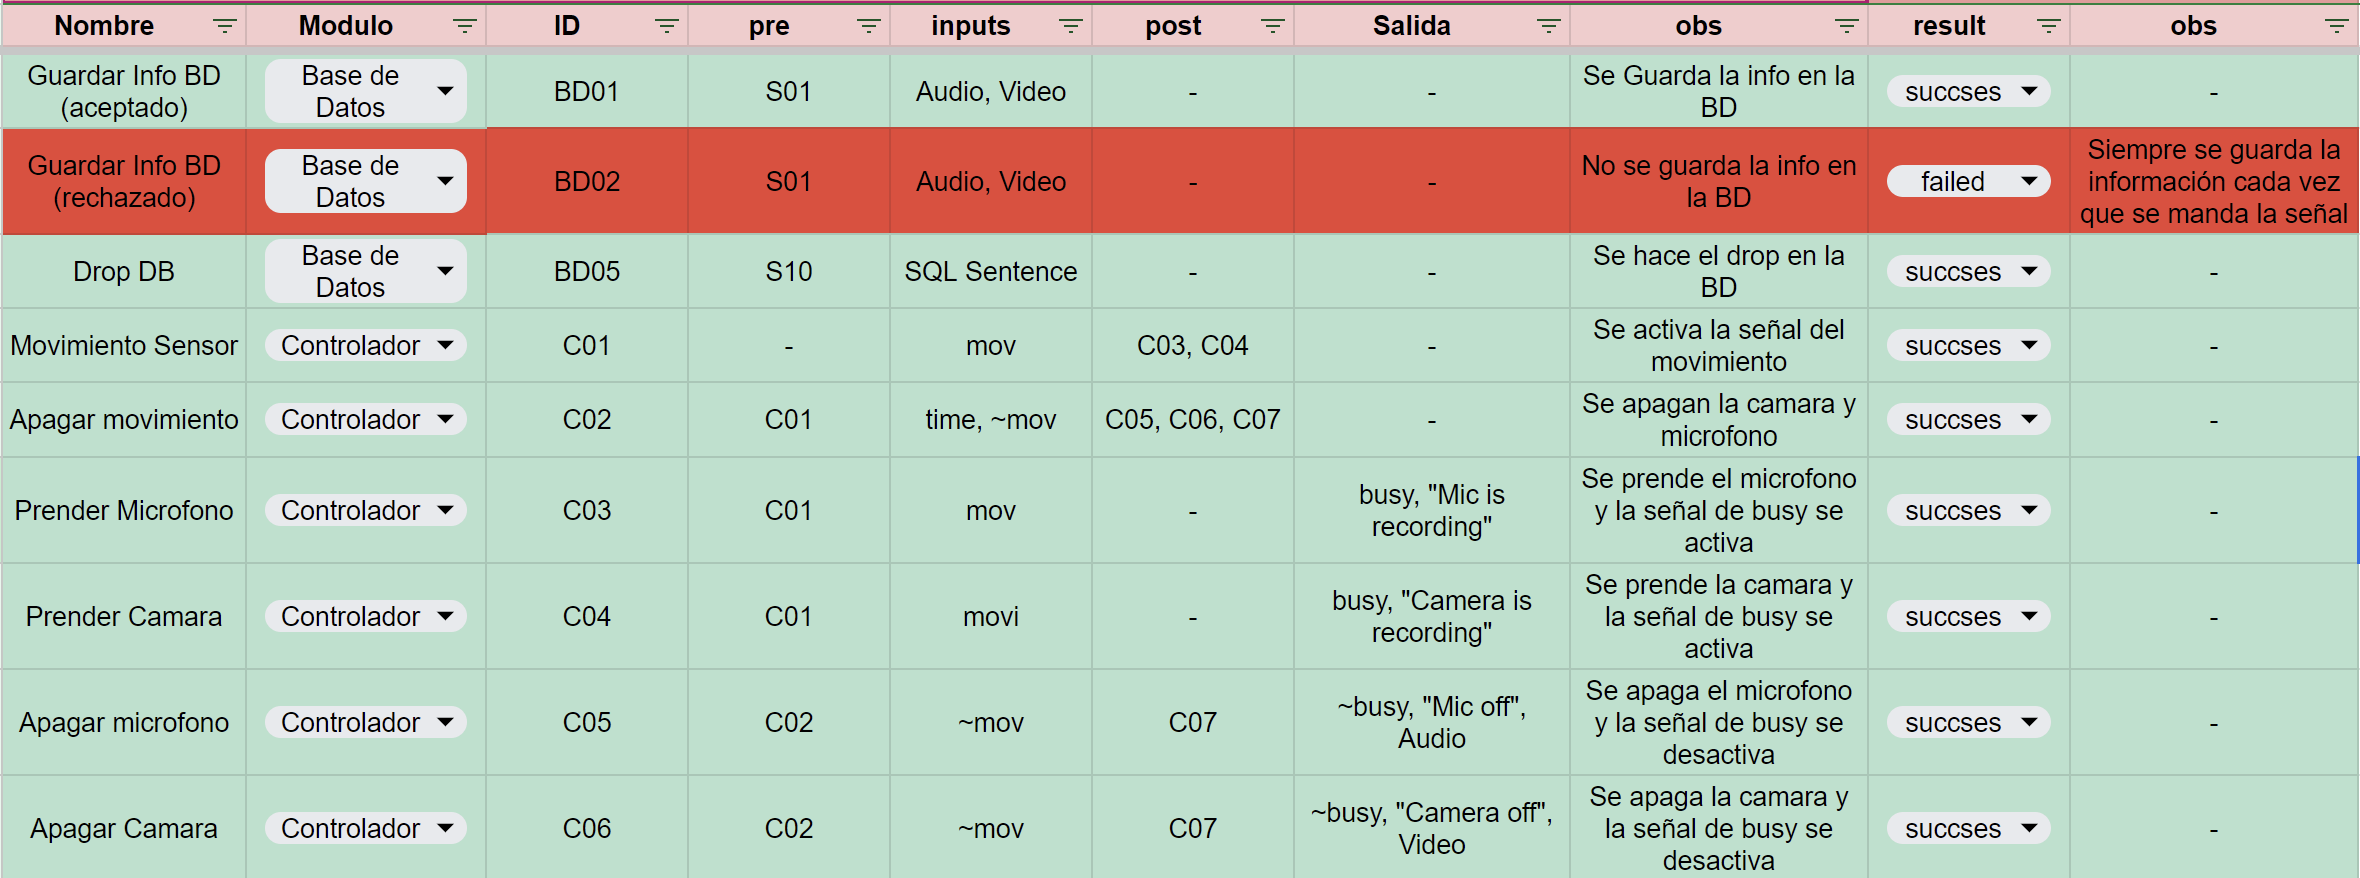
\includegraphics[width=16.5cm, height=7cm]{images/PDP1.PNG}
    \caption{Plan de Prueba 1/4}
    \label{fig:PDP1}
\end{figure}

\begin{figure}[!h]
    \centering
    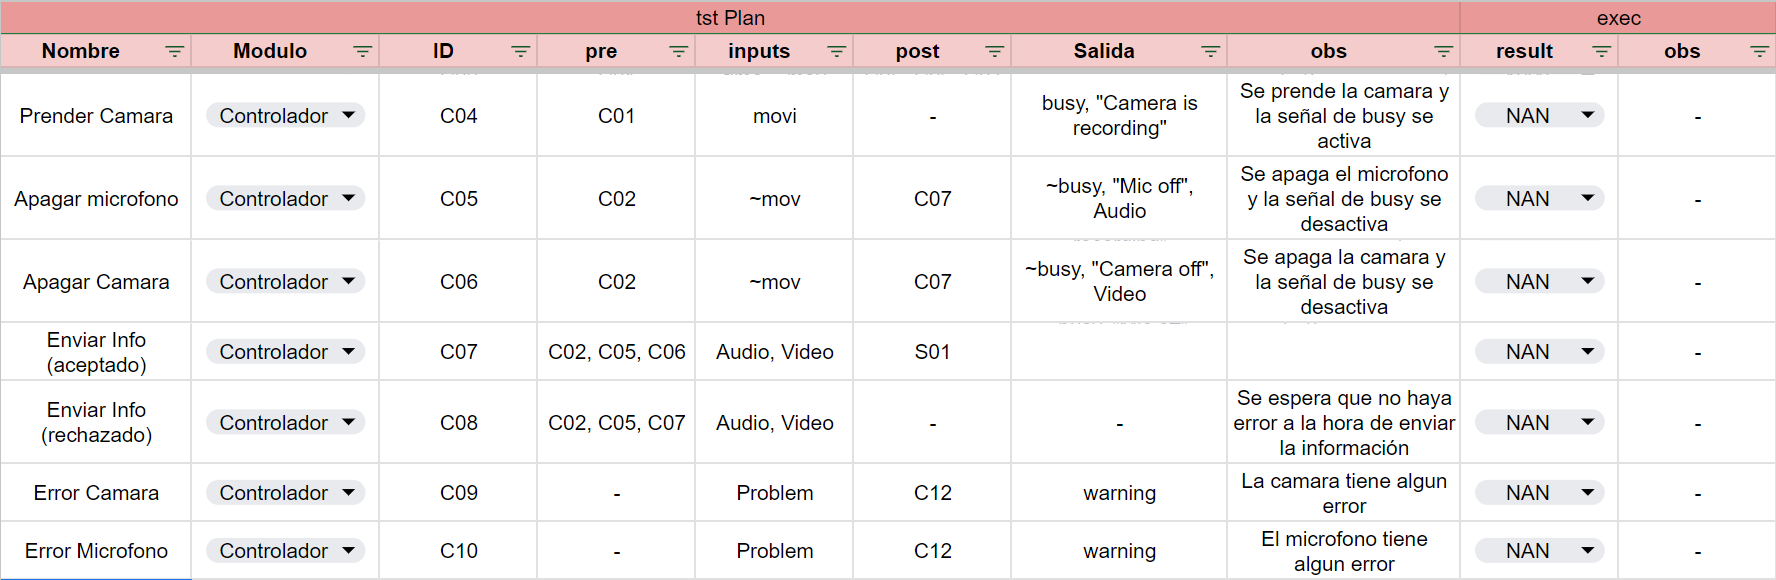
\includegraphics[width=16.5cm, height=6.5cm]{images/PDP2.PNG}
    \caption{Plan de Prueba 2/4}
    \label{fig:PDP2}
\end{figure}

\begin{figure}[!h]
    \centering
    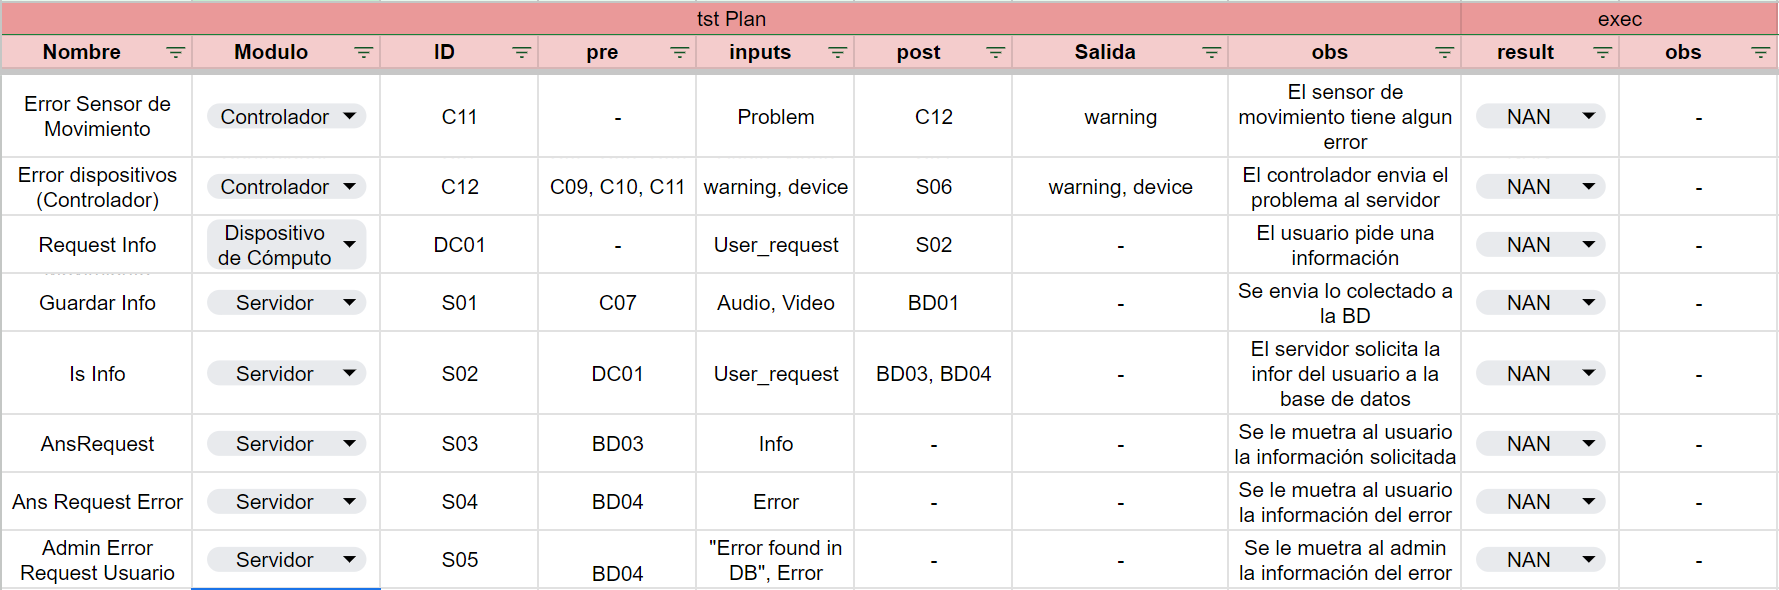
\includegraphics[width=16.5cm, height=6.5cm]{images/PDP3.PNG}
    \caption{Plan de Prueba 3/4}
    \label{fig:PDP3}
\end{figure}

\begin{figure}[!h]
    \centering
    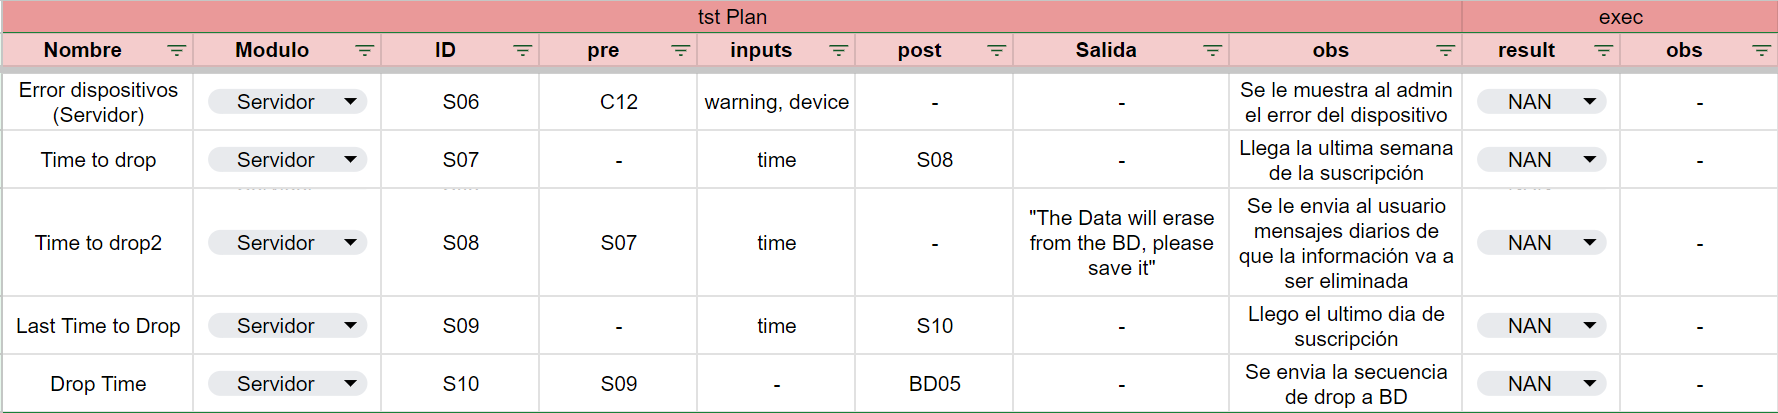
\includegraphics[width=16.5cm, height=5.5cm]{images/PDP4.PNG}
    \caption{Plan de Prueba 4/4}
    \label{fig:PDP4}
\end{figure}

%%==================================================================================
\pagebreak
\section{Prototipado en C}

Para el proyecto se realizó un primer prototipo en el lenguaje C con diferentes hilos de procesamiento. Estos hilos se separaron en las diferentes funcionalidades del proyectos, dichas funcionalidades fueron divididas en 8 módulos (tabla \ref{tab:modulos}), donde cada módulo tiene sus estados y señales (mensajes), los cuales fueron de utilidad para poder realizar la comunicación entre los hilos. Para dicha comunicación se creó una cola de mensajes que permitió encolar hasta ocho diferentes instrucciones. 

\begin{table}[!h]
\centering
\begin{tabular}{|c|c|}
\hline
\rowcolor[HTML]{C0C0C0} 
\textbf{Módulo} & \textbf{Tarea}                                                                                                         \\ \hline
pServer & \begin{tabular}[c]{@{}c@{}}Encargado de la comunicación\\ entre el usuario y la información\\ recolectada por los dispositivos.\end{tabular} \\ \hline
pCamera         & Controlador de la cámara                                                                                               \\ \hline
pMicro          & Controlador del micrófono                                                                                              \\ \hline
pMoveSensor     & \begin{tabular}[c]{@{}c@{}}Controlador del sensor de\\ movimientos\end{tabular}                                        \\ \hline
pController     & \begin{tabular}[c]{@{}c@{}}Controlador general de los \\ dispositivos de recolección de\\ información\end{tabular}     \\ \hline
pDatabase       & \begin{tabular}[c]{@{}c@{}}Comunicación con la\\ Base de Datos\end{tabular}                                            \\ \hline
pAdmin          & \begin{tabular}[c]{@{}c@{}}Módulo del administrador del\\ sistema para el monitoreo de los\\ dispositivos\end{tabular} \\ \hline
pNube           & \begin{tabular}[c]{@{}c@{}}Módulo de comunicación en la\\ nube\end{tabular}                                            \\ \hline
\end{tabular}
\caption{Hilos del sistema}
\label{tab:modulos}
\end{table}

Para la realización del proyecto se desarrollaron unas señales. Cada señal se envía por los canales que conectan los procesos con la finalidad de realizar ciertos tipos de acciones y enviar mensajes, donde algunas de estas señales llevan información a través de parámetros. Toda esta información se puede visualizar en la tabla \ref{tab:mensajes_info} a modo de resumen para visualizar las señales que se usaron en la elaboración del prototipo del sistema. Estas señales se crearon al seguir los diagramas SDL. 


\begin{table}[!h]
\centering
\resizebox{\textwidth}{!}{%
\begin{tabular}{|l|l|l|l|}
\hline
\textbf{TO\_DEVICES\_SIGNAL} & \textbf{TO\_DEVICES}              & \textbf{TO\_SERVER\_BD}           & \textbf{TO\_BD\_CLOUD}  \\ \hline
turnOn                       & sendInfo(const char*)             & requestInfo(const char*)          & ansRequest(const char*) \\ \hline
turnOff                      & move(integer)                     & errorFound                        & dropData                \\ \hline
move\_detected(integer)      & busy                              & tiempo(integer)                   &                         \\ \hline
error(const char*, const char*)           & warning(const char*, const char*) & answer(integer) &                         \\ \hline
                             &                                   & info1             &                         \\ \hline
                             &                                   & td                                &                         \\ \hline
                             &                                   & lt                                &                         \\ \hline
                             &                                   & isInfo(const char*)               &                         \\ \hline

\end{tabular}%
}
\caption{Mensajes del sistema con sus parámetros}
\label{tab:mensajes_info}
\end{table}
\pagebreak

Dentro del código se uso una estructura para la realización del paso de mensaje a través de los distintos canales. Esta estructura se compuso de cuatro atributos. El primer atributo fue el nombre de la señal identificado por el nombre signal. El segundo atributo fue un valor numérico para aquellas señales que envían un entero como tipo de dato indentificado como value. El tercera atributo fue el nombre del dispositivo como una cadena de caracteres (este atributo es importante para la señal de warning en el canal TO\_DEVICES y la señal de error en el canal TO\_DEVICES\_SIGNAL) identificado como device. Por ultimo, el cuarto atributo fue una información en formato de cadena de texto identificado como info. 

\begin{lstlisting}[style=C]
typedef struct {
  int signal;
  int value;
  char device[20];
  char info[150];
} msg_t;
\end{lstlisting}

Para una segunda entrega del prototipo se pudo visualizar una mejora con respecto a esta estructura. Para ello, se piensa realizar un cambio en el segundo atributo value para que este sea un tipo de dato void*. De esta manera el valor podrá tomar cualquier tipo de dato (la identificación del tipo de dato se hará a través del nombre de la señal). Para aquellas señales que usan mas de un parámetro se piensa realizar una estructura con dos atributos correspondientes al dispositivo y la información. 

\begin{lstlisting}[style=C]
typedef struct {
  int signal;
  void* value;
} msg_t;

typedef struct {
  char device[20];
  char info[150];
} Info_Data;

\end{lstlisting}

Después de haber finalizado de escoger la estructura que represento a los mensajes dentro del prototipo, se prosiguió a codificar las señales con un valor numérico. Como resultado de la codificación se obtuvo los valores descritos en la tabla \ref{tab:senales_sistema}.

\begin{table}[!h]
\resizebox{\textwidth}{!}{%
\begin{tabular}{|l|l|l|l|}
\hline
\textbf{TO\_DEVICES\_SIGNAL} & \textbf{TO\_DEVICES} & \textbf{TO\_SERVER\_BD} & \textbf{TO\_BD\_CLOUD} \\ \hline
turnOn (0)                   & sendInfo (0)         & requestInfo (0)         & ansRequest (0)         \\ \hline
turnOff (1)                  & move (1)             & errorFound (1)          & dropData (1)           \\ \hline
move\_detected (2)           & busy (2)             & tiempo (2)              &                        \\ \hline
error(3)                     & warning (3)          & answer (3)              &                        \\ \hline
                             &                      & info1 (4)            &                        \\ \hline
                             &                      & td (5)                  &                        \\ \hline
                             &                      & lt (6)                  &                        \\ \hline
                             &                      & isInfo (7)              &                        \\ \hline

\end{tabular}%
}
\caption{Señales del sistema con su identificador en el código}
\label{tab:senales_sistema}
\end{table}
\pagebreak

El siguiente paso en la elaboración del prototipo fue la codificación de los estados dentro de los procesos. Previamente, en el SDL, en la comunicación del sistema se pudo observar la creación de estados dentro de los procesos. Para la elaboración de dichos estados, se crearon seis estructuras dentro del prototipo que permitieron seguir el flujo de trabajo establecido en los diagramas. Es importante recalcar que tres de los procesos del prototipo comparten la misma funcionalidad, por esto no se elaboraron ocho estructuras de estados. Para este paso, también se realizó una codificación que se puede observar en las tablas \ref{tab:estados1} y \ref{tab:estados2}.

\begin{table}[!h]
\resizebox{\textwidth}{!}{%
\begin{tabular}{|l|l|l|}
\hline
\textbf{PROCESO\_CONTROLADOR\_STATES} & \textbf{PROCESO\_SERBDNUBE\_STATES} & \textbf{PROCESO\_DEVICES\_STATES} \\ \hline
Comunicaciones\_dispocontro (0)      & Comunicaciones\_serBDNube (0)      & Comunicaciones\_devices (0)      \\ \hline
Apagar (1)                          & RecibirRes (1)                    &                                 \\ \hline
Prender (2)                         & Respuesta (2)                     &                                 \\ \hline
RecibirInfo (3)                     & DevolverInfo (3)                  &                                 \\ \hline
                                    & DevolverErrores (4)               &                                 \\ \hline
\end{tabular}%
}
\caption{Estados del sistema 1/2}
\label{tab:estados1}
\end{table}

\begin{table}[!h]
\resizebox{\textwidth}{!}{%
\begin{tabular}{|l|l|l|}
\hline
\textbf{PROCESO\_ACCIONES\_STATES} & \textbf{PROCESO\_ADMIN\_STATES} & \textbf{PROCESO\_BD\_STATES} \\ \hline
Comunicaciones\_acciones (0)       & Comunicaciones\_admin (0)       & Comunicaciones\_bd (0)       \\ \hline
                                   &                                 &                              \\ \hline
                                   &                                 &                              \\ \hline
                                   &                                 &                              \\ \hline
                                   &                                 &                              \\ \hline
\end{tabular}%
}
\caption{Estados del sistema 2/2}
\label{tab:estados2}
\end{table}

Finalmente, se realizo el código de los ocho módulos definidos en la tabla \ref{tab:modulos}, siguiendo los diagramas SDL desarrollados.